\section{eo\-One\-Max\-Quad\-Crossover$<$ Genotype\-T $>$ Class Template Reference}
\label{classeo_one_max_quad_crossover}\index{eoOneMaxQuadCrossover@{eoOneMaxQuadCrossover}}
Always write a comment in this format before class definition if you want the class to be documented by Doxygen.  


{\tt \#include $<$eo\-One\-Max\-Quad\-Crossover.h$>$}

Inheritance diagram for eo\-One\-Max\-Quad\-Crossover$<$ Genotype\-T $>$::\begin{figure}[H]
\begin{center}
\leavevmode
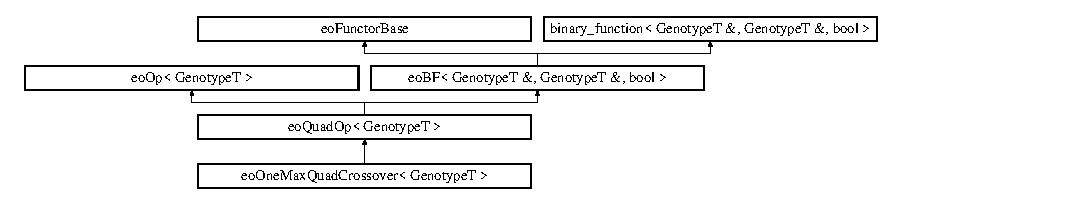
\includegraphics[height=2.30453cm]{classeo_one_max_quad_crossover}
\end{center}
\end{figure}
\subsection*{Public Member Functions}
\begin{CompactItemize}
\item 
{\bf eo\-One\-Max\-Quad\-Crossover} ()\label{classeo_one_max_quad_crossover_a0}

\begin{CompactList}\small\item\em Ctor - no requirement. \item\end{CompactList}\item 
string {\bf class\-Name} () const \label{classeo_one_max_quad_crossover_a1}

\begin{CompactList}\small\item\em The class name. Used to display statistics. \item\end{CompactList}\item 
bool {\bf operator()} (Genotype\-T \&\_\-genotype1, Genotype\-T \&\_\-genotype2)
\begin{CompactList}\small\item\em eo\-Quad crossover - modifies both parents \item\end{CompactList}\end{CompactItemize}


\subsection{Detailed Description}
\subsubsection*{template$<$class Genotype\-T$>$ class eo\-One\-Max\-Quad\-Crossover$<$ Genotype\-T $>$}

Always write a comment in this format before class definition if you want the class to be documented by Doxygen. 

THere is NO ASSUMPTION on the class Genoype\-T. In particular, it does not need to derive from {\bf EO}{\rm (p.\,\pageref{class_e_o})} 



Definition at line 26 of file eo\-One\-Max\-Quad\-Crossover.h.

\subsection{Member Function Documentation}
\index{eoOneMaxQuadCrossover@{eo\-One\-Max\-Quad\-Crossover}!operator()@{operator()}}
\index{operator()@{operator()}!eoOneMaxQuadCrossover@{eo\-One\-Max\-Quad\-Crossover}}
\subsubsection{\setlength{\rightskip}{0pt plus 5cm}template$<$class Genotype\-T$>$ bool {\bf eo\-One\-Max\-Quad\-Crossover}$<$ Genotype\-T $>$::operator() (Genotype\-T \& {\em \_\-genotype1}, Genotype\-T \& {\em \_\-genotype2})\hspace{0.3cm}{\tt  [inline, virtual]}}\label{classeo_one_max_quad_crossover_a2}


eo\-Quad crossover - modifies both parents 

\begin{Desc}
\item[Parameters:]
\begin{description}
\item[{\em \_\-genotype1}]The first parent \item[{\em \_\-genotype2}]The second parent\end{description}
\end{Desc}


Requirement if (at least one genotype has been modified) // no way to distinguish one\-At\-Least\-Is\-Modified = true; else one\-At\-Least\-Is\-Modified = false; 

Implements {\bf eo\-BF$<$ Genotype\-T \&, Genotype\-T \&, bool $>$} {\rm (p.\,\pageref{classeo_b_f_a1})}.

Definition at line 49 of file eo\-One\-Max\-Quad\-Crossover.h.

The documentation for this class was generated from the following file:\begin{CompactItemize}
\item 
eo\-One\-Max\-Quad\-Crossover.h\end{CompactItemize}
